
\chapter{Selección de variables de análisis y proceso de estudio}
\label{cha:seleccion de variables de analisis y proceso de estudio}

Tras la sinopsis de herramientas de \emph{web scraping} de código abierto, se pretende realizar una 
introducción al proceso de evaluación de las mismas. El capítulo se dividirá en tres secciones claramente 
diferenciadas las cuales se especifican con más detalle a continuación:

\begin{enumerate}
  \item En primer lugar se realiza una introducción sobre el proceso de evaluación a realizar. ¿Cuáles
  son los aspectos más importantes en la evaluación de herramientas de minería web? ¿Es posible realizar 
  una valoración objetiva entre bibliotecas de diferentes lenguajes de programación?
  \item La segunda sección trata sobre el proceso de comparación, así como una introducción al código
  desarrollado para este. El proceso de tokenización y la creación/comparación de n-gramas o bloques son 
  algunos de los aspectos a destacar. ¿Cuál es el tamaño óptimo de cada n-grama o bloque? ¿Cómo se determina 
  si la extracción ha sido exitosa?
  \item Por último, se especifican las variables de comparación y los test preparados de cada algoritmo.
  Se determina el proceso seguido para calcular la precisión, velocidad de extracción, uso de memoria
  y demás características de cada algoritmo.
\end{enumerate}

Cabe destacar que la evaluación será conjunta, las herramientas de los diferentes lenguajes de programación 
serán sometidas a los mismos test con el fin de ver aquellas bibliotecas o paquetes más involucrados en el 
proceso de minado web. 

A lo largo del capítulo será posible comprobar en los diferentes fragmentos de código como se ha realizado
la integración de las diversas herramientas, y sobre como es posible construir una valoración objetiva para
cualquier herramienta de minado web desarrollada sobre cualquier lenguaje de programación convencional.

\section{Introducción al proceso de evaluación}
\label{sec:introduccion al proceso de evaluacion}

Cuando cualquier usuario entra en un sitio web lo que busca es obtener la información requerida lo más
rápido y preciso posible. La calidad del texto extraído es prioritaria, para ello el uso de heurísticas o
la eliminación de contenido \emph{boilerplate} es crucial en cualquier algoritmo de \emph{web scraping}.

Muchos de los algoritmos descartados para el proceso de evaluación como \textbf{scrapeR}, o ni si quiera 
mencionados en la sinopsis de paquetes como \textbf{selectr} \cite{selectr}, emplean únicamente expresiones 
regulares para la extracción de contenido. Esto provoca que la extracción de texto no sea 'limpia', puesto 
que siempre van a existir resultados donde se extraiga contenido no deseado.

El objetivo de este proyecto concierne la evaluación del proceso heurístico de las diferentes herramientas
de minado web. La inclusión de algoritmos que emplean únicamente expresiones XPath o selectores CSS no
tiene sentido para la herramienta desarrollada, pues cualquier analizador de los ya mencionados en el
apéndice \ref{cha:analizadores empleados en los paquetes de web scraping} podría realizar el mismo trabajo.

\subsection{Aspectos generales a considerar}
\label{subsec:aspectos generales a considerar}

La gran mayoría de los \emph{web scrapers} son capaces de extraer fragmentos de información de un sitio
web, ya sea el precio de un determinado producto en venta, el autor de un ensayo o el resultado de un 
partido de fútbol. Pero además, se espera que estas herramientas de minado puedan ser una solución fiable 
y de calidad con respecto a la extracción tradicional, ¿es posible medir de algún modo la calidad del texto 
extraído de estas herramientas?

La respuesta es si, y para ello, los algoritmos se centrarán en la extracción de artículos de prensa en su
mayoría, con el objetivo de que estos sean comparados con un texto base. Se define como texto base aquellos 
fragmentos de texto principal de cualquier sitio web que el usuario visualizaría al entrar. Se muestra en 
la figura \ref{img:estructura generica del proceso de evaluacion} la estructura general del proceso de 
evaluación.

\begin{figure}[tphb]
  \centering
  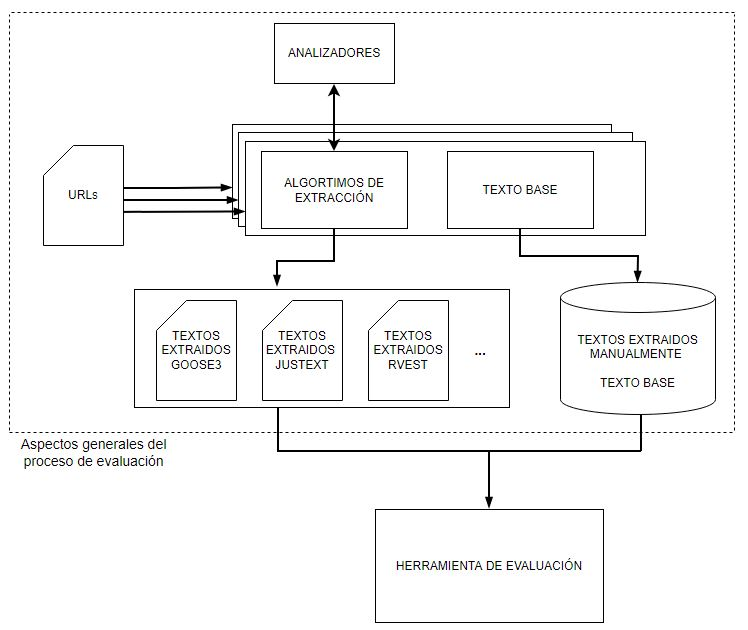
\includegraphics[width=5in]{estructura-generica-proceso-evaluacion.jpg}
  \caption{Estructura genérica del proceso de evaluación}
  \label{img:estructura generica del proceso de evaluacion}
\end{figure}

Tanto los textos obtenidos por los algoritmos de \emph{web scraping}, como los textos producidos por la 
extracción manual, se almacenan de forma ordenada en archivos JSON con el objetivo de que su acceso sea 
sencillo para cualquier lenguaje de programación.

\subsection{Cuerpo principal del sitio web como objetivo de la evaluación}
\label{subsec:cuerpo principal del sitio web como objetivo de la evaluacion}

Como ya se ha mencionado anteriormente, una de las características más importantes de un \emph{web scraper}
es la capacidad de extraer de texto de calidad. Por lo tanto, comparar el texto extraído de diferentes
algoritmos será el cometido de la herramienta de evaluación. Ahora la principal pregunta es, ¿qué fragmentos
de texto son considerados como principales?

Imaginemos un artículo web de noticias tradicional o una entrada de blog, algo parecido a lo mostrado en
la figura \ref{img:articulo web tradicional}, del que se pretende extraer
información de valor. En la imagen se reflejan varias secciones claramente diferenciadas, anuncios de
contenidos relacionados, información de autor e incluso elementos de navegación.

\begin{figure}[tphb]
  \centering
  
\includegraphics[width=6in]{pagina-web.jpeg}
  \caption{Artículo web tradicional}
  \label{img:articulo web tradicional}
\end{figure}

La tarea de extracción puede parecer sencilla, pero dependiendo del sitio web puede ser sorprendentemente
complicada y llena de matices \cite{boilerplate-removal}. La selección del cuerpo principal del sitio web 
será el objetivo de cada algoritmo. Para conseguir un cuerpo de artículo no solo será necesario saber dónde 
empieza o termina este, también se deberán conocer las partes a excluir. 

Con el fin de la que la evaluación sea lo más justa posible, se debe definir qué compone el cuerpo del
artículo, y estar seguros de que todas las herramientas siguen los mismos objetivos. El principio subyacente 
es que el cuerpo del artículo debe ser un texto limpio, sin campos adicionales, elementos de navegación o 
anuncios. En la siguiente lista se determina el conjunto de elementos o secciones de un sitio web no 
contemplados en la evaluación:

\begin{itemize}
  \item Campos de información sobre autor/es, fechas de publicación, palabras clave o títulos de imágenes 
  y vídeos.
  \item Botones para compartir y sugerencias para compartir un artículo, artículos relacionados, enlaces 
  'leer a continuación', 'recomendado para usted'...
  \item Comentarios e interfaz de usuario relacionada con los mismos. Elementos de navegación propios del
  sitio web.
  \item Elementos de control alrededor de las imágenes que producen texto innecesario, número de imágenes
  en una galería, botones superpuestos a una imagen/vídeo...
  \item Código JavaScript. Aunque esta no sea una sección específica de un sitio web, muchas herramientas
  extraen estos fragmentos de código pensado que pertenece como parte del contenido principal del propio 
  artículo.
\end{itemize}

Se muestra a continuación la lista de elementos que serán extraídos por las diferentes herramientas como
parte del contenido principal, ademas del propio contenido principal.

\begin{itemize}
  \item Título principal de artículo.
  \item Enlaces para leer con más detalle, a la fuente u otros contenidos directamente relacionados. Estos 
  enlaces pueden requerir un conocimiento mucho más profundo y complejo del contenido principal del sitio 
  web.
  \item Avisos de copyright.
\end{itemize}

En definitiva, todo fragmento que pueda ser extraído y comparado con el original y del que se puedan obtener 
conclusiones firmes, será incluido como parte del contenido principal. Véase la figura 
\ref{img:contenido boilerplate de un articulo web tradicional} en la que se determinan las secciones 
descartadas y definidas como contenido \emph{boilerplate} o 'basura'.

\begin{figure}[tphb]
  \centering
  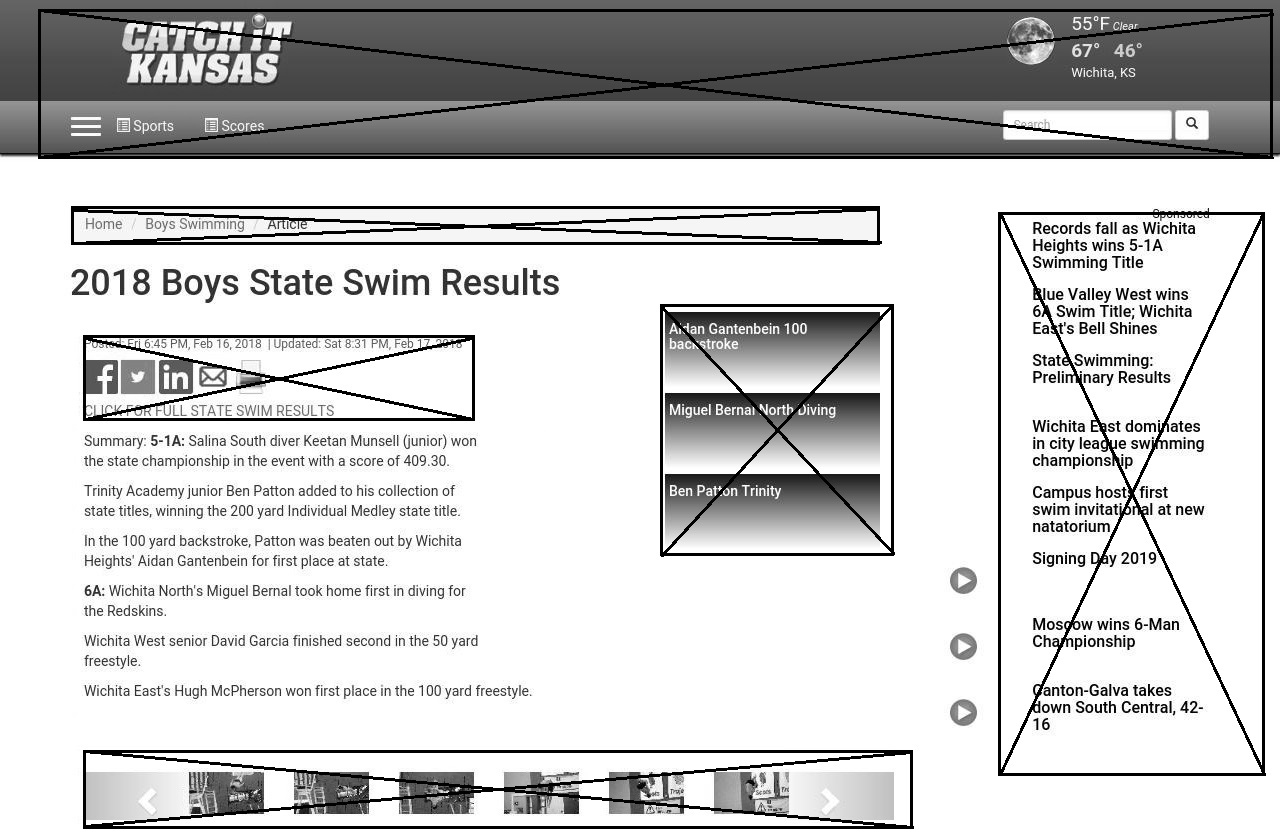
\includegraphics[width=6.1in]{pagina-web2.jpeg}
  \caption{Contenido \emph{boilerplate} de un artículo web tradicional}
  \label{img:contenido boilerplate de un articulo web tradicional}
\end{figure}

\subsection{Recopilación del conjunto de datos}
\label{subsec:recopilacion del conjunto de datos}

Una vez definido en que consiste el cuerpo principal de cada artículo, el siguiente paso consiste en la
recolección del conjunto de datos de prueba para la herramienta. Se pretende que este conjunto sea diverso, 
representativo e imparcial. Es por ello que en el \emph{dataset} no solo se compone artículos de noticias 
relevantes, también hay un conjunto muy variado de artículos no informativos como entradas de blog, 
comunicados de prensa...

El proceso de recolección del conjunto de datos consiste en tomar una muestra aleatoria del millón de
sitios web escritos en inglés. Para cada sitio, se comprueba si contiene algún artículo, en cuyo caso, se
añaden dos de ellos al azar. En una primera instancia, el conjunto que compone el \emph{dataset} suponía
cerca de 200 sitios web listos para analizar.

Antes de comenzar con el proceso de evaluación se deben asegurar una serie de conceptos relacionados con
posibles errores de acceso, análisis o extracción de la información de algunas de las páginas incluidas:

\begin{enumerate}
  \item Se debe asegurar que las páginas no cambian durante el análisis. Minimizar las posibilidades de 
  obtener un artículo actualizado durante la extracción.
  \item Se deben excluir aquellas páginas que las herramientas no sean capaces de descargar.
  \item Se deben descartar aquellas paginas cuyo contenido no sea explícitamente escrito en inglés.
\end{enumerate}

Tras tener en cuenta todas estas consideraciones, el grupo inicial de 200 páginas se redujo a 101 casos
listos para el análisis. Aún realizada la reducción, el \emph{dataset} es lo suficientemente amplio como
para sacar conclusiones claras de los algoritmos a analizar.

Por último, como ya se ha mencionado anteriormente, tanto la información extraída de forma manual, como
aquella extraída por los algoritmos de minado web, es almacenada en archivos JSON. Esto hace mucho más
cómodo el análisis, pues el acceso a cada texto es mucho más sencillo. Se muestra a continuación un ejemplo
de como se almacenan los diferentes textos extraídos por \textbf{BeautifulSoup}.

\begin{Schunk}
  \begin{Soutput}
  {
    "0000test": {
        "texto": "Nadal keeps Spain alive against Russia in Davis Cup Finals..."
    },
    ...
    "0100test": {
        "texto": "CNN - Breaking News, Latest News and Videos CNN | 11/25/2021..."
    }
  }
  \end{Soutput}
\end{Schunk}

De la misma forma se almacenan los textos extraídos de forma manual. En este caso, se guarda información
adicional del sitio web. Como se puede observar, el orden de almacenamiento es clave, pues de él depende
que el análisis sea correcto.

\begin{Schunk}
  \begin{Soutput}
  {
    "0000test": {
        "texto": "MADRID — Rafael Nadal kept Spain’s hopes alive, then Marcel...",
        "url": "https://www.sportsnet.ca/tennis/..."
    },
    ...
    "0100test": {
      "texto": "Groups of thieves target two high-end stores in California...",
      "url": "http://lite.cnn.com/en/article/..."
    }
  }
  \end{Soutput}
\end{Schunk}

Esta forma de almacenamiento es aplicada a todos los algoritmos de minado, no solo a aquellos desarrollados
en Python, las herramientas codificadas en R también lo aplican. Esto permite incluir en la evaluación a
cualquier algoritmo de minado web desarrollado sobre un lenguaje de programación que permita trabajar con
documentos JSON.

\section{Análisis de la herramienta de evaluación}
\label{sec:analisis de la herramienta de evaluacion}

Una vez se dispone del \emph{dataset} al completo, el objetivo es comparar cada uno de los textos obtenidos
por las herramientas de extracción con el texto base. La exposición de las diferentes soluciones aportadas
será clave para comprender el resultado final.

Uno de los aspectos fundamentales de la herramienta de evaluación es su heurística. Se debe pensar en un
algoritmo que sea capaz de comparar diferentes tipos de textos minimizando la probabilidad de fallo. A lo
largo de la sección se mostrará como el proceso no es sencillo pues muchos algoritmos de extracción
presentan diferentes soluciones a un mismo problema.

\begin{figure}[tphb]
  \centering
  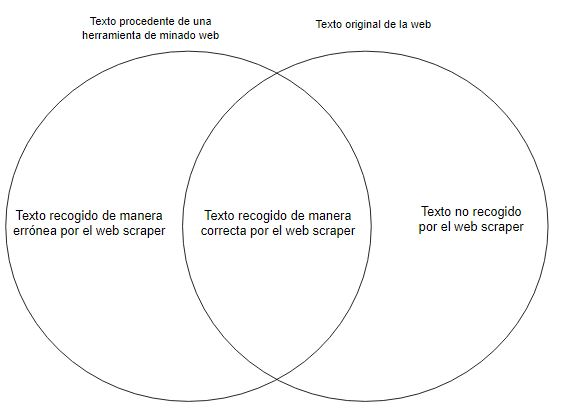
\includegraphics[width=5in]{diagrama-venn.jpg}
  \caption{Diagrama de Venn: Texto base vs texto extraído}
  \label{img:diagrama venn: texto base vs texto extraido}
\end{figure}

La principal preocupación subyace por la forma en la que los diferentes algoritmos consideran como parte
de contenido principal de un sitio web. En algunas ocasiones es posible configurar la manera de extracción
de los mismos, pero en otra no. Es por ello que se debe pensar en un método lo suficientemente justo como
para comparar múltiples textos de diversas procedencias que pueden ser ligeramente diferentes.

\subsection{Aspectos específicos a considerar}
\label{subsec:aspectos especificos a considerar}

En la figura \ref{img:estructura generica del proceso de evaluacion} se definía de forma genérica como se
gestionaba la información recogida por los diferentes algoritmos de \emph{web scraping}. Veamos ahora como
se trata y se compara dicha información con la extraída manualmente con el objetivo de conocer aquellos
algoritmos que más se acercan a un resultado real.

\begin{figure}[tphb]
  \centering
  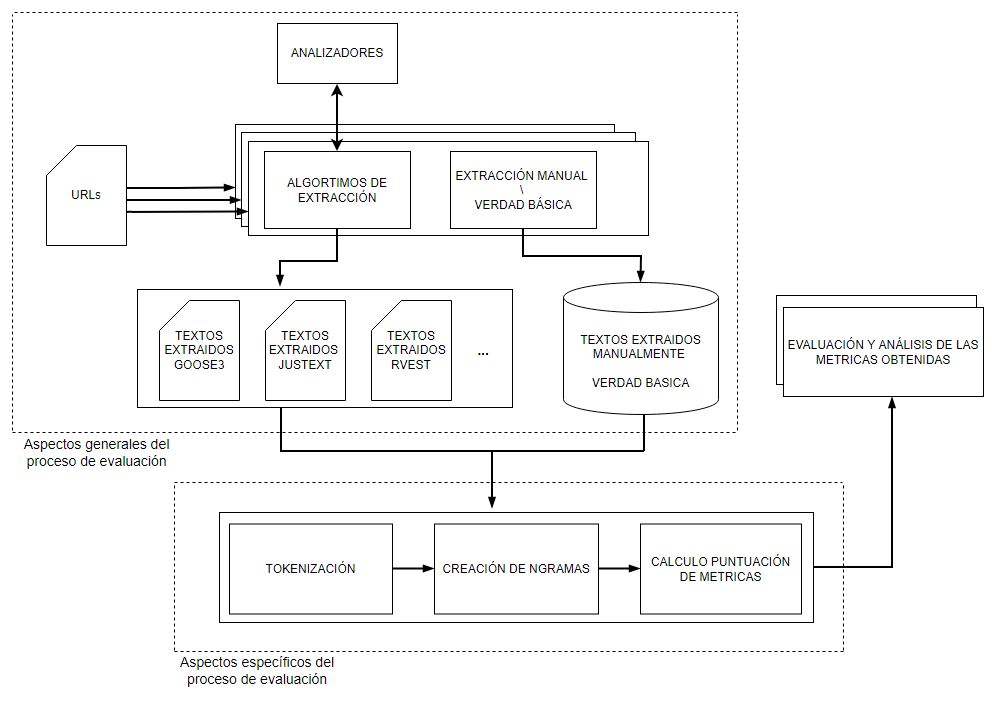
\includegraphics[width=7.1in]{estructura-especifica-proceso-evaluacion.jpg}
  \caption{Estructura especifica del proceso de evaluación}
  \label{img:estructura específica del proceso de evaluacion}
\end{figure}

Se puede observar en la figura \ref{img:estructura específica del proceso de evaluacion} la solución
adoptada por la herramienta de evaluación. Tras la obtención de texto base y texto extraído, se pretende
realizar un proceso de tokenización y creación de n-gramas, clave a la hora de realizar el posterior cálculo
de métricas. En cuanto a la evaluación y análisis de métricas obtenidas, se abordará en el próximo capítulo.

\subsection{Heurística basada en n-gramas}
\label{subsec:heuristica basada en n-gramas}

A lo largo de la sección se aborda el problema de comparar diferentes fragmentos de texto. Se presentan
diferentes soluciones, una de ellas podría ser la comparación de palabras en la misma posición, otra podría
ser la búsqueda de palabras pertenecientes a ambos textos. Veamos porque la división en n-gramas es un
buen método para este propósito.

\subsubsection{Comparación de texto empleando el método palabra por posición}
\label{subsubsec:comparacion de textos empleando el metodo palabra por posicion}

Imaginemos que se disponen dos textos a comparar como los siguientes. El primero de ellos se considera como
texto base, pues ha sido obtenido de forma manual del propio sitio web. El segundo surge como resultado 
de la ejecución de cualquiera de las herramientas de \emph{web scraping} expuestas en el capítulo anterior.

\begin{Schunk}
  \begin{Soutput}
      MADRID — Top-ranked Rafael Nadal has arrived in Madrid to
      lead Spain in the new-look Davis Cup Finals.\n\n\"It’s a
      new competition and we must be focused,\" Nadal said Sunday.

      MADRID \u2014 Top-ranked Rafael Nadal has arrived in Madrid to 
      lead Spain in the new-look Davis Cup Finals.\"It\u2019s a 
      new competition and we must be focused,\" Nadal said Sunday.
  \end{Soutput}
\end{Schunk}

Veamos el funcionamiento de los diferentes métodos de comparación pensados. En primer lugar, se aplica la
comparación palabra por palabra, donde se prepara un fragmento de código que recorra ambos textos al mismo
tiempo y determine si las palabras dispuestas en la misma posición son idénticas.

\begin{figure}[tphb]
  \centering
  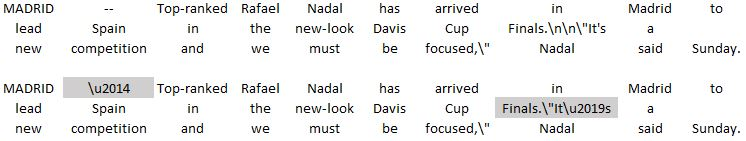
\includegraphics[width=6.5in]{text-comparison1.jpg}
  \caption{Comparación de textos empleando el método palabra por posición}
  \label{img:comparacion de textos empleando el metodo palabra por posicion}
\end{figure}

Como se muestra en la figura \ref{img:comparacion de textos empleando el metodo palabra por posicion} la 
comparación no ha sido tan desastrosa como se esperaba. Los únicos errores han sido producidos por espacios 
en blanco y caracteres Unicode que la herramienta de minado web no ha sido capaz de detectar.

El problema con esta solución viene cuando la disposición de los mismos no es exacta, o incluso cuando 
ambos fragmentos no tienen el mismo tamaño. Imaginemos que la herramienta de minado no ha sido capaz de 
detectar la palabra \textbf{MADRID} como parte del contenido principal. En este caso, ninguna palabra 
coincidiría con la original pues las posiciones no están dispuestas del mismo modo.

\begin{figure}[tphb]
  \centering
  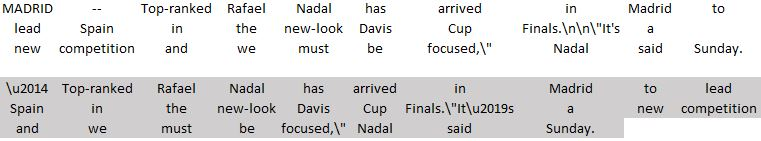
\includegraphics[width=6.5in]{text-comparison2.jpg}
  \caption{Comparación de textos empleando el método palabra por posición}
  \label{img:comparacion de textos empleando el metodo palabra por posicion p2}
\end{figure}

Esta forma de comparación no funcionaria, y menos en artículos donde los fragmentos de textos son amplios
y las posibilidades de fallo aumentan. Además, el \emph{dataset} es de gran volumen por lo que la posibilidad 
de que existan fragmentos de texto con disposiciones totalmente distintas a la original tiene una alta 
probabilidad.

\subsubsection{Comparación de texto empleando el método palabra por detección}
\label{subsubsec:comparacion de textos empleando el metodo palabra por deteccion}

Es necesario encontrar entonces en una nueva heurística que minimice la probabilidad de fallo, donde la 
posición de cada palabra no sea un aspecto a tener en cuenta. Una solución podría darse con el recorrido 
de uno de los fragmentos de texto, donde se busquen palabras coincidentes con el otro. Se selecciona una 
palabra pivote, por ejemplo \textbf{Spain}, y se recorre el segundo texto hasta encontrar la palabra 
indicada.

\begin{figure}[tphb]
  \centering
  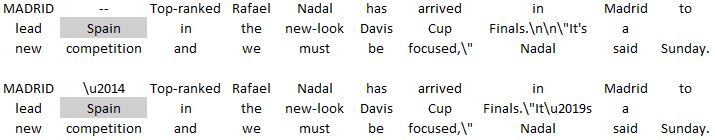
\includegraphics[width=6.5in]{text-comparison3.jpg}
  \caption{Comparación de textos empleando el método palabra por detección}
  \label{img:comparacion de textos empleando el metodo palabra por deteccion}
\end{figure}

En realidad, si se realiza un análisis profundo sobre esta solución, surgen nuevas problemáticas. ¿Qué
ocurriría si apareciesen dos palabras idénticas sobre el mismo texto? Imaginemos que durante el recorrido
del primer texto, se debe analizar una palabra pivote repetida varias veces a lo largo del segundo texto. 
La heurística anterior no sería correcta, veamos un ejemplo.

Comienza el algoritmo seleccionando pivotes y realizando la heurística correspondiente para cada uno, 
primero con \textbf{MADRID}, luego con \textbf{'--'}, y así sucesivamente hasta llegar a \textbf{Nadal} 
que es el que nos interesa en este ejemplo. Se recorre el segundo fragmento buscado dicha palabra y se 
encuentran dos apariciones de la misma. Para ambas apariciones se calcula y se suma una puntuación 
determinada.

\begin{figure}[tphb]
  \centering
  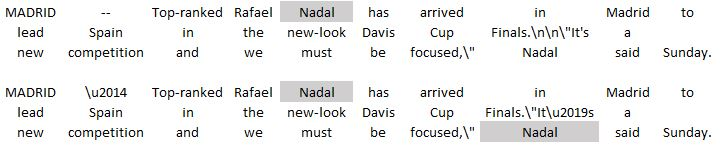
\includegraphics[width=6.5in]{text-comparison4.jpg}
  \caption{Comparación de textos empleando el método palabra por detección}
  \label{img:comparacion de textos empleando el metodo palabra por deteccion p2}
\end{figure}

El algoritmo sigue realizando el bucle y nuevamente emplea la palabra \textbf{Nadal} como pivote, pero en
este caso en su segunda aparición. Se volvería a efectuar un calculo y la posterior suma de su puntuación.
La implementación de esta heurística forzaría un resultado irreal, pues este error se acrecentaría sobre
\emph{datasets} extensos que contengan fragmentos de texto prolongados, como es el caso.

\begin{figure}[tphb]
  \centering
  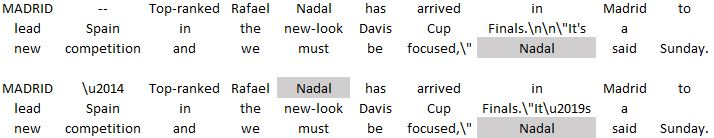
\includegraphics[width=6.5in]{text-comparison5.jpg}
  \caption{Comparación de textos empleando el método palabra por detección}
  \label{img:comparacion de textos empleando el metodo palabra por deteccion p3}
\end{figure}

\subsubsection{Comparación de texto empleando la creacion de n-gramas}
\label{subsubsec:comparacion de textos empleando la creacion de n-gramas}

Se debe pensar entonces en una nueva heurística que nuevamente minimice la probabilidad de fallo, la cual
tenga en cuenta que la posición de cada palabra debe ser irrelevante y que cuide la posible repetición de
palabras. Se utilizan bloques como estructuras de datos, veamos como funciona.

Los bloques o n-gramas se consideran conjuntos de secuencias alfanuméricas, en las que se descartan los
espacios en blanco y se separan los signos de puntuación \cite{ngrams-thesis}. Esto funciona bien en la 
mayoría de los casos, ya que normalmente el texto a excluir se encuentra en bloques separados por nuevas 
líneas o espacios en blanco. Siguiendo con el ejemplo anterior, la división de texto en n-gramas donde 
\emph{n = 3} sería:

\begin{figure}[tphb]
  \centering
  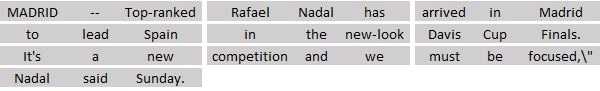
\includegraphics[width=6in]{text-comparison6.jpg}
  \caption{Creación de n-gramas}
  \label{img:creacion de n-gramas}
\end{figure}

El objetivo ahora es separar ambos textos en n-gramas de tamaño \emph{n} y realizar la comparación entre
ellos. La posición ya no es relevante pues la comparación no se va a ejecutar en torno a la posición de cada
n-grama. Además, la repetición de n-gramas no es preocupante pues existe una baja probabilidad de que esto
ocurra a lo largo del texto.

\begin{figure}[tphb]
  \centering
  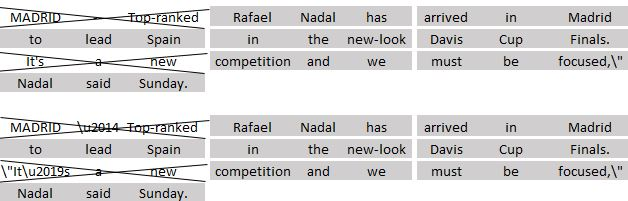
\includegraphics[width=6in]{text-comparison7.jpg}
  \caption{Comparación de textos empleando n-gramas}
  \label{img:comparacion de textos empleando n-gramas p2}
\end{figure}

El algoritmo procede del mismo modo que antes, se selecciona un n-grama pivote y se buscan n-gramas
coincidentes en el texto extraído. Tras el recorrido completo del texto se determina una cierta puntuación.
En la figura \ref{img:comparacion de textos empleando n-gramas p2} se muestra el resultado de ejecución
del algoritmo.

Si observamos de nuevo la figura anterior, los n-gramas en séptima y primera posición del texto base no 
coincide con los n-gramas del texto extraído, a pesar de que la mayor parte de las palabras sí que son 
coincidentes. Es posible realizar una mejora dividiendo el texto en el mayor número de n-gramas posibles. 
Este aumento de divisiones se efectúa con el objetivo de recuperar la mayor cantidad de palabras mejorando 
así la precisión de la herramienta desarrollada.

\begin{codefloat}
  \inputencoding{latin1}
  \lstinputlisting[style=CppExample, showstringspaces=false]{scripts/evaluacion-tokenizar.py}
  \inputencoding{utf8}
  \caption{Proceso de tokenización}
  \label{cod:proceso de tokenizacion}
\end{codefloat}

En los fragmentos de código \ref{cod:proceso de tokenizacion} y
\ref{cod:creacion de n-gramas a partir de los tokens resultantes} se muestra el proceso de tokenización y
creación de n-gramas usado en la herramienta de evaluación. Para el desarrollo de la herramienta se ha
decidido emplear n-gramas donde \emph{n = 4} con el objetivo de aumentar la precisión del resultado dado.

\begin{codefloat}
  \inputencoding{latin1}
  \lstinputlisting[style=CppExample, showstringspaces=false]{scripts/evaluacion-ngramas.py}
  \inputencoding{utf8}
  \caption{Creación de n-gramas a partir de los tokens resultantes}
  \label{cod:creacion de n-gramas a partir de los tokens resultantes}
\end{codefloat}

Aplicando esta metodología al ejemplo anterior se obtienen una cantidad bastante mayor de n-gramas. Este
mismo proceso se realiza tanto en el texto base, como en el texto extraído, para poder realizar el cálculo
posterior de la puntuación.

\begin{Schunk}
  \begin{Soutput}
(MADRID -- Top-ranked Rafael), (-- Top-ranked Rafael Nadal), 
(Top-ranked Rafael Nadal has), (Rafael Nadal has arrived), 
(Nadal has arrived in), (has arrived in Madrid), (arrived in Madrid to), 
(in Madrid to lead), (Madrid to lead Spain), (to lead Spain in), 
(lead Spain in the), (Spain in the new-look), (in the new-look Davis), 
(the new-look Davis Cup), (new-look Davis Cup Finals.), (Davis Cup Finals. It’s),
(Cup Finals. It’s a), (Finals. It’s a new), (It’s a new competition),
(a new competition and), (new competition and we), (competition and we must), 
(and we must be), (we must be focused,), (must be focused, Nadal),
(be focused, Nadal said), (focused, Nadal said Sunday.)
  \end{Soutput}
\end{Schunk}

\subsection{Cálculo y puntuación de n-gramas}
\label{subsec:calculo y puntuacion de n-gramas}

Una vez que ambos fragmentos de texto han sido convertidos en n-gramas, se debe realizar el cálculo del
texto extraído para poder conocer la calidad del mismo. Para comprender como se ha desarrollado dicho
cálculo, debemos recordar la figura \ref{img:diagrama venn: texto base vs texto extraido}, donde el 
diagrama de Venn expuesto representa los tres posibles tipos de puntuaciones.

Para realizar el cálculo y puntuación de n-gramas, se desarrolla un clasificador binario, encargado de 
realizar una clasificación de instancias positivas y negativas:

\begin{itemize}
  \item Positivo: La instancia se clasifica como miembro de la clase que el clasificador está tratando de 
  identificar. Por ejemplo, un clasificador que busque fotos de gatos clasificará las fotos con gatos como 
  positivas cuando sean correctas.
  \item Negativo: La instancia se clasifica como no perteneciente a la clase que se intenta identificar. 
  Por ejemplo, un clasificador que busque fotos de gatos debería clasificar las fotos con perros como 
  negativas.
\end{itemize}

Las bases de las métricas independientes del entorno de ejecución especificadas en la sección
\ref{subsubsec:metricas independientes del entorno de ejecucion}, provienen de los conceptos de 
\textbf{True Positive}, \textbf{False Positive} y \textbf{False Negative}. La tabla 
\ref{tab:ejemplos de instancias positivas y negativas} ilustra estos conceptos, donde se considera el 
valor '1' como una predicción positiva.

\begin{table}[h]
  \begin{center}
  \begin{tabular}{| c | c | c | c |} \hline
  \textbf{Predicción} & \textbf{Valor actual} & \textbf{Tipo} & \textbf{Explicación}\\ \hline
  1 & 1 & True Positive & La predicción coincidió con el valor resultante \\ \hline
  1 & 0 & False Positive & La predicción no coincidió con el valor resultante \\ \hline
  0 & 1 & False Negative & La predicción no coincidió con el valor resultante \\ \hline
  \end{tabular}
  \caption{Ejemplos de instancias positivas y negativas}
  \label{tab:ejemplos de instancias positivas y negativas}
  \end{center}
\end{table}

Una instancia que no se tiene en cuenta en el clasificador desarrollado para el cálculo de métricas es 
\textbf{True Negative}. Esta instancia determinaría la capacidad de la herramienta para clasificar contenido 
que no se ha predicho. Se muestran algunos ejemplos en la tabla \ref{tab:ejemplos de true negative}.

\begin{table}[h]
  \begin{center}
  \begin{tabular}{| c | c | c | c |} \hline
  \textbf{Predicción} & \textbf{Valor actual} & \textbf{Tipo} & \textbf{Explicación}\\ \hline
  0 & 0 & True Negative & La predicción coincidió con el valor resultante \\ \hline
  No Gato & No Gato & True Negative & Se predijo que no había gato y no era un gato \\ \hline
  (Nadal Rafael has) & (Nadal Rafael has) & True Negative & Se predijo n-grama erróneo y era erróneo \\ \hline
  \end{tabular}
  \caption{Ejemplos de True Negative}
  \label{tab:ejemplos de true negative}
  \end{center}
\end{table}

Los n-gramas que coinciden en el texto base y en el texto extraído se conoce como \textbf{True Positives}.
Se muestra en el fragmento de código \ref{cod:calculo de true positives} como se realiza dicho cálculo.

\begin{codefloat}
  \inputencoding{latin1}
  \lstinputlisting[style=CppExample, showstringspaces=false]{scripts/evaluacion-true-positives.py}
  \inputencoding{utf8}
  \caption{Cálculo de true positives}
  \label{cod:calculo de true positives}
\end{codefloat}

Por otro lado, los n-gramas que aparecen en el texto extraído, pero no en el texto base se conoce como 
\textbf{False Positives}. Se muestra en el fragmento de código \ref{cod:calculo de false positives} como 
se realiza dicho cálculo.

\begin{codefloat}
  \inputencoding{latin1}
  \lstinputlisting[style=CppExample, showstringspaces=false]{scripts/evaluacion-false-positives.py}
  \inputencoding{utf8}
  \caption{Cálculo de false positives}
  \label{cod:calculo de false positives}
\end{codefloat}

Por ultimo, los n-gramas que aparecen en el texto base pero no en el texto extraído se conoce como 
\textbf{False Negatives}. Se muestra en el fragmento de código \ref{cod:calculo de false negatives} como 
se realiza dicho cálculo.

\begin{codefloat}
  \inputencoding{latin1}
  \lstinputlisting[style=CppExample, showstringspaces=false]{scripts/evaluacion-false-negatives.py}
  \inputencoding{utf8}
  \caption{Cálculo de false negatives}
  \label{cod:calculo de false negatives}
\end{codefloat}

Una vez conocidas estas tres posibles puntuaciones, lo único que se debe hacer es recorrer el texto base
y texto extraído, haciendo una comparación de n-gramas. El código fragmento de código mostrado en
\ref{cod:calculo de puntuaciones} se encarga de retornar una tupla con las puntuaciones calculadas.

\begin{codefloat}
  \inputencoding{latin1}
  \lstinputlisting[style=CppExample, showstringspaces=false]{scripts/evaluacion-puntuacion.py}
  \inputencoding{utf8}
  \caption{Cálculo de puntuaciones}
  \label{cod:calculo de puntuaciones}
\end{codefloat}

Con el objetivo de esclarecer como funciona el cálculo de la puntuación, se emplea el ejemplo anterior
como sujeto de pruebas. Se muestra a continuación el texto base y extraído convertidos en n-gramas donde 
\emph{n = 4}.

\begin{figure}[tphb]
  \centering
  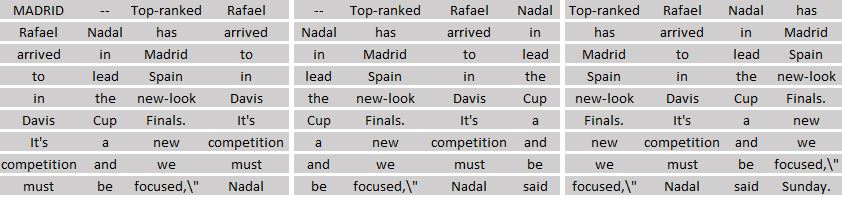
\includegraphics[width=6.3in]{text-comparison8.jpg}
  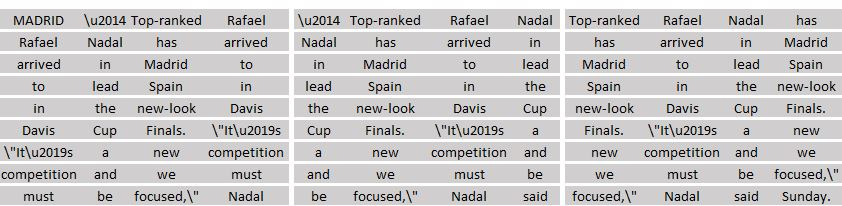
\includegraphics[width=6.3in]{text-comparison9.jpg}
  \caption{Comparación de textos empleando n-gramas mejorados}
  \label{img:comparacion de textos empleando n-gramas mejorados}
\end{figure}

Una vez aplicada la heurística habitual del algoritmo, se procede con el cálculo de la puntuación. Se
realiza el recorrido de n-gramas de ambos textos y se va realizando el cálculo. Se muestran las puntuaciones 
calculadas la matriz de confusión \ref{img:matriz de confusion de las instancias calculadas}.

\begin{figure}[tphb]
  \centering
  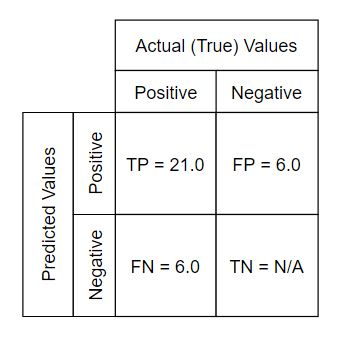
\includegraphics[width=4.5in]{matriz-confusion.jpg}
  \caption{Matriz de confusión de las instancias calculadas}
  \label{img:matriz de confusion de las instancias calculadas}
\end{figure}

Una vez realizado el cálculo de las diferentes instancias, se procede con las métricas. Algunos términos 
básicos son \textbf{Precision}, \textbf{Recall} y \textbf{F1-Score}. Estos términos están relacionados con 
lo bien que funciona un clasificador, en lugar de limitarse a observar la precisión general.

\subsection{Introducción a las métricas de evaluación}
\label{subsec:introduccion a las metricas de evaluacion}

Una vez realizado todo el proceso heurístico y el posterior cálculo de puntuaciones, se debe medir como de
buenos son los diferentes algoritmos de extracción. Se propone efectuar una división de métricas, por un
lado, se determinarán métricas que dependan del entorno en el que se ejecute el programa, por otro lado,
se definirán otras métricas no dependientes de dicho entorno. 

Por otro lado, es conveniente revisar el apéndice \ref{cha:metricas descartadas del proceso de evaluacion},
donde se especifican métricas adicionales que finalmente han sido descartadas. Su descarte, es debido a su 
poca implicación en la evaluación o por el reemplazo de otras métricas más desarrolladas.

\subsubsection{Métricas independientes del entorno de ejecución}
\label{subsubsec:metricas independientes del entorno de ejecucion}

En esta sección, se determinan las diferentes métricas que definirán la calidad de extracción de cada 
algoritmo. Se definen como métricas independientes del entorno, porque no dependen del medio de ejecución, 
ni del lenguaje de programación usado para dicho procedimiento.

En la figura \ref{img:jerarquia de metricas} se muestra la jerarquía existente entre el cálculo de instancias
y métricas. A primera vista, es una red un poco desordenada. Las métricas forman una jerarquía que comienza
con las negativas/positivas, y que llega hasta la puntuación F1 para unirlas todas. Estas métricas son 
dependientes de las instancias previamente calculadas.

\begin{figure}[tphb]
  \centering
  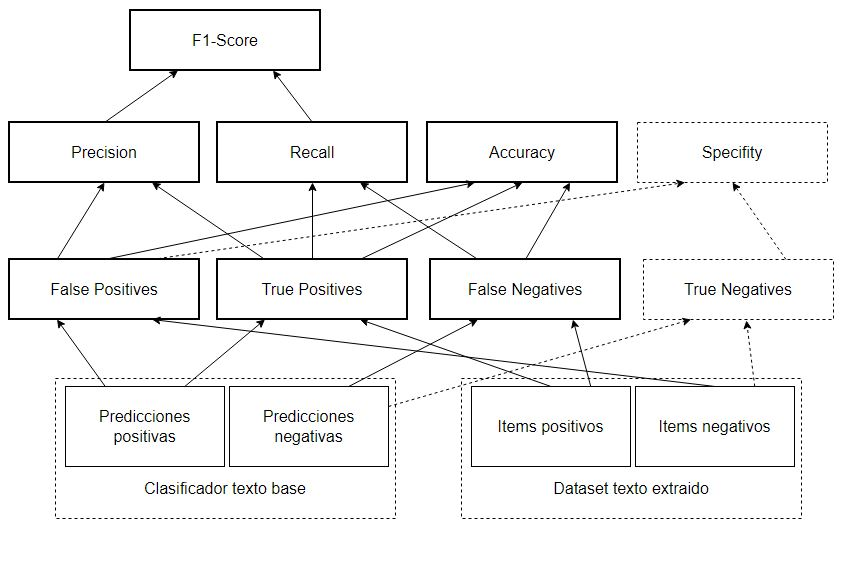
\includegraphics[width=6.5in]{estructura-metricas.jpg}
  \caption{Jerarquía de métricas}
  \label{img:jerarquia de metricas}
\end{figure}

La primera métrica se conoce como \emph{precision}, y mide el número de predicciones positivas realizadas
que son correctas. En otras palabras, mide la eficacia de los sistemas para excluir contenido
\emph{boilerplate} de un sitio web. A continuación se determina tanto la formula para su cálculo, como el
fragmento de código incluido en la herramienta de evaluación.

\begin{equation*}
  Precision = \frac{True\;Positives}{True\;Positives + False\;Positives} = 
  \frac{N.\;of\;Correctly\;Predicted\;Positive\;Instances}{N.\;of\;Total\;Positives\;Predictions\;you\;Made}
\end{equation*}

\begin{codefloat}
  \inputencoding{latin1}
  \lstinputlisting[style=CppExample, showstringspaces=false]{scripts/evaluacion-precision.py}
  \inputencoding{utf8}
  \caption{Cálculo de la métrica \emph{precision}}
  \label{cod:calculo de la metrica precision}
\end{codefloat}

Otra de las métricas obligadas a calcular es lo que se conoce como \emph{recall}. Esta característica mide
el número de casos positivos que el clasificador predijo correctamente, sobre todos los casos positivos del
\emph{dataset}. A veces también se denomina \emph{sensitivity}. En términos generales, mide la eficacia de
los sistemas para captar las partes deseadas del cuerpo del artículo. En el fragmento de código
\ref{cod:calculo de la metrica recall} se muestra como se realiza el cálculo.

\begin{equation*}
  Recall = \frac{True\;Positives}{True\;Positives + False\;Negatives} = 
  \frac{N.\;of\;Correctly\;Predicted\;Positive\;Instances}{N.\;of\;Total\;Positives\;Intances\;in\;the\;Dataset}
\end{equation*}

\begin{codefloat}
  \inputencoding{latin1}
  \lstinputlisting[style=CppExample, showstringspaces=false]{scripts/evaluacion-recall.py}
  \inputencoding{utf8}
  \caption{Cálculo de la métrica \emph{recall}}
  \label{cod:calculo de la metrica recall}
\end{codefloat}

Tanto la \emph{precision} como \emph{recall} son métricas importantes de analizar, puesto que miden como
de bien diferencian el contenido importante del contenido \emph{boilerplate} los diferentes algoritmos de
\emph{web scraping}. Estas métricas definen la manera en la que los algoritmos siguen lo especificado en
la sección \ref{subsec:cuerpo principal del sitio web como objetivo de la evaluacion}.

Combinando ambas métricas es posible determinar la calidad en general de la extracción. Esta característica
se denomina F1, y funciona bien en los casos en los que los conjuntos de datos están desequilibrados,
ya que requiere que tanto las métricas de \emph{precision} como \emph{recall} tengan un valor razonable.

\begin{equation*}
  F1 = 2 * \frac{precision * recall}{precision + recall}
\end{equation*}

Por último, se realiza el cálculo de lo que se conoce como \emph{accuracy}, la cual mide la proporción de
predicciones correctas sobre el número total de predicciones. A continuación se muestra tanto la fórmula
de cálculo, como su implementación en el entorno de evaluación.

\begin{equation*}
  Accuracy = \frac{True\;Positives}{True\;Positives + False\;Negatives + False\;Positives} = 
  \frac{N.\;of\;Correct\;Predictions}{N.\;of\;All\;Predictions}
\end{equation*}

\begin{codefloat}
  \inputencoding{latin1}
  \lstinputlisting[style=CppExample, showstringspaces=false]{scripts/evaluacion-accuracy.py}
  \inputencoding{utf8}
  \caption{Cálculo de la métrica \emph{accuracy}}
  \label{cod:calculo de la metrica accuracy}
\end{codefloat}

\subsubsection{Métricas dependientes del entorno de ejecución}
\label{subsubsec:metricas dependientes del entorno de ejecucion}

A lo largo de esta sección, se especificarán aspectos relativos al rendimiento a la hora de utilizar 
\emph{web scraping} como un posible sustituto de la extracción tradicional. Aspectos como la gestión de 
recursos no se tienen en cuenta en un principio, pero pueden ser cruciales a la hora de realizar minado web 
sobre múltiples documentos \cite{emil-persson}.

Antes de comenzar con el cálculo de métricas, es conveniente asegurar la integridad de la evaluación. Al
trabajar con múltiples lenguajes de programación pueden existir conflictos, ya sean relacionados con la 
complejidad de los algoritmos o con las bibliotecas empleadas.

El primer aspecto a considerar tiene que ver con el diseño de los algoritmos. Aquellos algoritmos escritos 
en diferentes lenguajes de programación deben presentar similitudes estructurales en su código. En los 
fragmentos \ref{cod:funcion de ejecucion de boilerpy} y \ref{cod:funcion de ejecucion de boilerpiper} 
se refleja claramente este aspecto.

\begin{codefloat}
  \inputencoding{latin1}
  \lstinputlisting[style=CppExample, showstringspaces=false]{scripts/script-boilerpy.py}
  \inputencoding{utf8}
  \caption{Función de ejecución de Boilerpy}
  \label{cod:funcion de ejecucion de boilerpy}
\end{codefloat}

\begin{codefloat}
  \inputencoding{latin1}
  \lstinputlisting[style=CppExample, showstringspaces=false]{scripts/script-boilerpiper.R}
  \inputencoding{utf8}
  \caption{Función de ejecución de BoilerpipeR}
  \label{cod:funcion de ejecucion de boilerpiper}
\end{codefloat}

En términos referentes a la complejidad, ambos algoritmos presentan una complejidad lineal. El número de
ejecuciones de ambos fragmentos de código dependerá del conjunto de elementos del \emph{dataset} de prueba,
pero siempre será finito.

Otro aspecto importante corresponde con el uso de herramientas referentes al cálculo de métricas. El empleo
de múltiples bibliotecas para abordar este aspecto afectaría negativamente a la integridad de la evaluación. 
Por ello se propone la utilización de una única interfaz entre lenguajes que unifique el proceso.

Para abordar esta problemática se pretende emplear la biblioteca \textbf{rpy2} \cite{rpy2} como interfaz 
entre ambos lenguajes. Esto permitirá que el compilador de Python ejecute líneas de código escritas en R. 
De esta forma, una misma biblioteca podrá monitorear algoritmos escritos en ambos lenguajes.

Resueltas ambas cuestiones, se procede con el cálculo. Para este propósito se emplean dos bibliotecas, por
un lado, \textbf{psutil} \cite{psutil} encargada de la supervisión del sistema y limitación de recursos, 
entre otros, y por otro \textbf{time} que permite el registro del tiempo de ejecución, pues retorna el 
número de segundos transcurridos desde un cierto instante.

\begin{figure}[tphb]
  \centering
  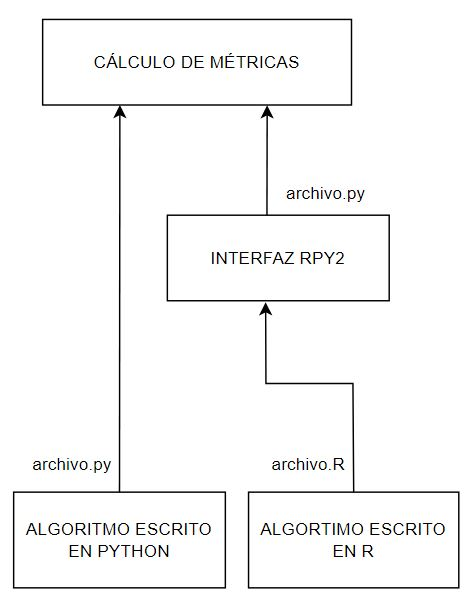
\includegraphics[width=3in]{estructura-interfaz-rpy2.jpg}
  \caption{Estructura del entorno de ejecución}
  \label{img:estructura del entorno de ejecucion}
\end{figure}

Se determinan a continuación las métricas seleccionadas, puesto que estas son dependientes del entorno de 
ejecución, los resultados diferirán según el medio en el que se realicen las pruebas. Se muestra en la
tabla \ref{tab:caracteristicas del entorno de ejecucion} las características del entorno empleado.

\begin{table}[h]
  \begin{center}
    \begin{tabular}{| c | c | c |} \hline 
     \textbf{Procesador (CPU)} & \textbf{Memoria RAM} & \textbf{Tarjeta Gráfica (GPU)} \\ \hline
     AMD Ryzen 7 2700 Eight-Core 3.20 GHz & 16,0 GB & NVIDIA GeForce RTX 2060 SUPER \\ \hline
    \end{tabular}
    \caption{Características del entorno de ejecución}
    \label{tab:caracteristicas del entorno de ejecucion}
  \end{center}
\end{table} 

\textbf{Tiempo de ejecución:}

La primera de las mediciones tiene que ver con el tiempo en realizar el proceso completo de minado. En el 
momento en el que el algoritmo comienza a extraer información se activa el contador, y este para cuando 
finaliza el proceso.

Cabe destacar que el cálculo de dicho tiempo abarca el proceso de minado al completo, desde el acceso al
contenido, hasta la transformación del mismo.

\textbf{Uso de CPU(\%):}

El uso de CPU es la cantidad total cantidad de procesador que consume la tarea a realizar. Permite valores 
por encima del 100\%, lo que indica que el proceso se ejecuta en múltiples hilos en diferentes núcleos de 
la CPU. La máquina que realizó las pruebas tiene un total de ocho núcleos, por lo que el 800\% significaría
que todos los núcleos trabajan al máximo en el proceso.

Para el cálculo del uso de CPU se emplea la función \emph{cpu\_percent(interval)}, que devuelve un número 
que representa la utilización actual de la CPU en todo el sistema en forma de porcentaje. Cuando la variable 
\emph{interval} es mayor que cero, compara los tiempos de CPU del sistema transcurridos antes y después de 
dicho intervalo.

\textbf{Uso de de memoria física o RAM(\%):}

La memoria real también conocida como memoria física o RAM, es la tercera métrica registrada. Simplemente 
mide la cantidad de memoria física que el proceso está empleando. Como recordatorio, la máquina en la que 
se realiza la evaluación tiene un total de 16GB de memoria física.

Para el cálculo del uso de memoria RAM se emplea la función \emph{virtual\_memory()}, que devuelve 
estadísticas sobre el uso de la memoria física total.





































